\section{Busca em árvore não-ordenada} \label{cap:3:section:btree}

\subsection{Introdução}

O algoritmo de busca em árvore não-ordenada funciona de modo que, eu atravesse todos
nós da minha árvore até que eu ache o elemento $x$ que está sendo buscado, se isso acontece
é retornado o nó que contém $x$.

\subsection{Implementação}

A implementação do algoritmo de busca em árvore não-ordenada consiste em atravessar todos os
nós da esquerda e depois os nós da direita, se o elemento é encontrado, ele é retornado de forma
recursiva.

\begin{lstlisting}[style=CStyle]
BinaryNode * search(BinaryNode * root, int key) 
{
    if (root == NULL || root->data == key) {
        return root;
    }

    BinaryNode * found = search(root->left, key);
    if (found == NULL) {
        found = search(root->right, key);
    }

    return found;
}
\end{lstlisting}
            

Seu tempo de execução é na ordem da equação \ref{cap:3:eq:bTree}.

\begin{equation} \label{cap:3:eq:bTree}
    T(n) = O(n)
\end{equation}

\subsection{Resultados}

Para a implementação, foi obtido o gráfico \ref{cap:3:graph:bTree}:

\begin{figure}[h]
    \centering
    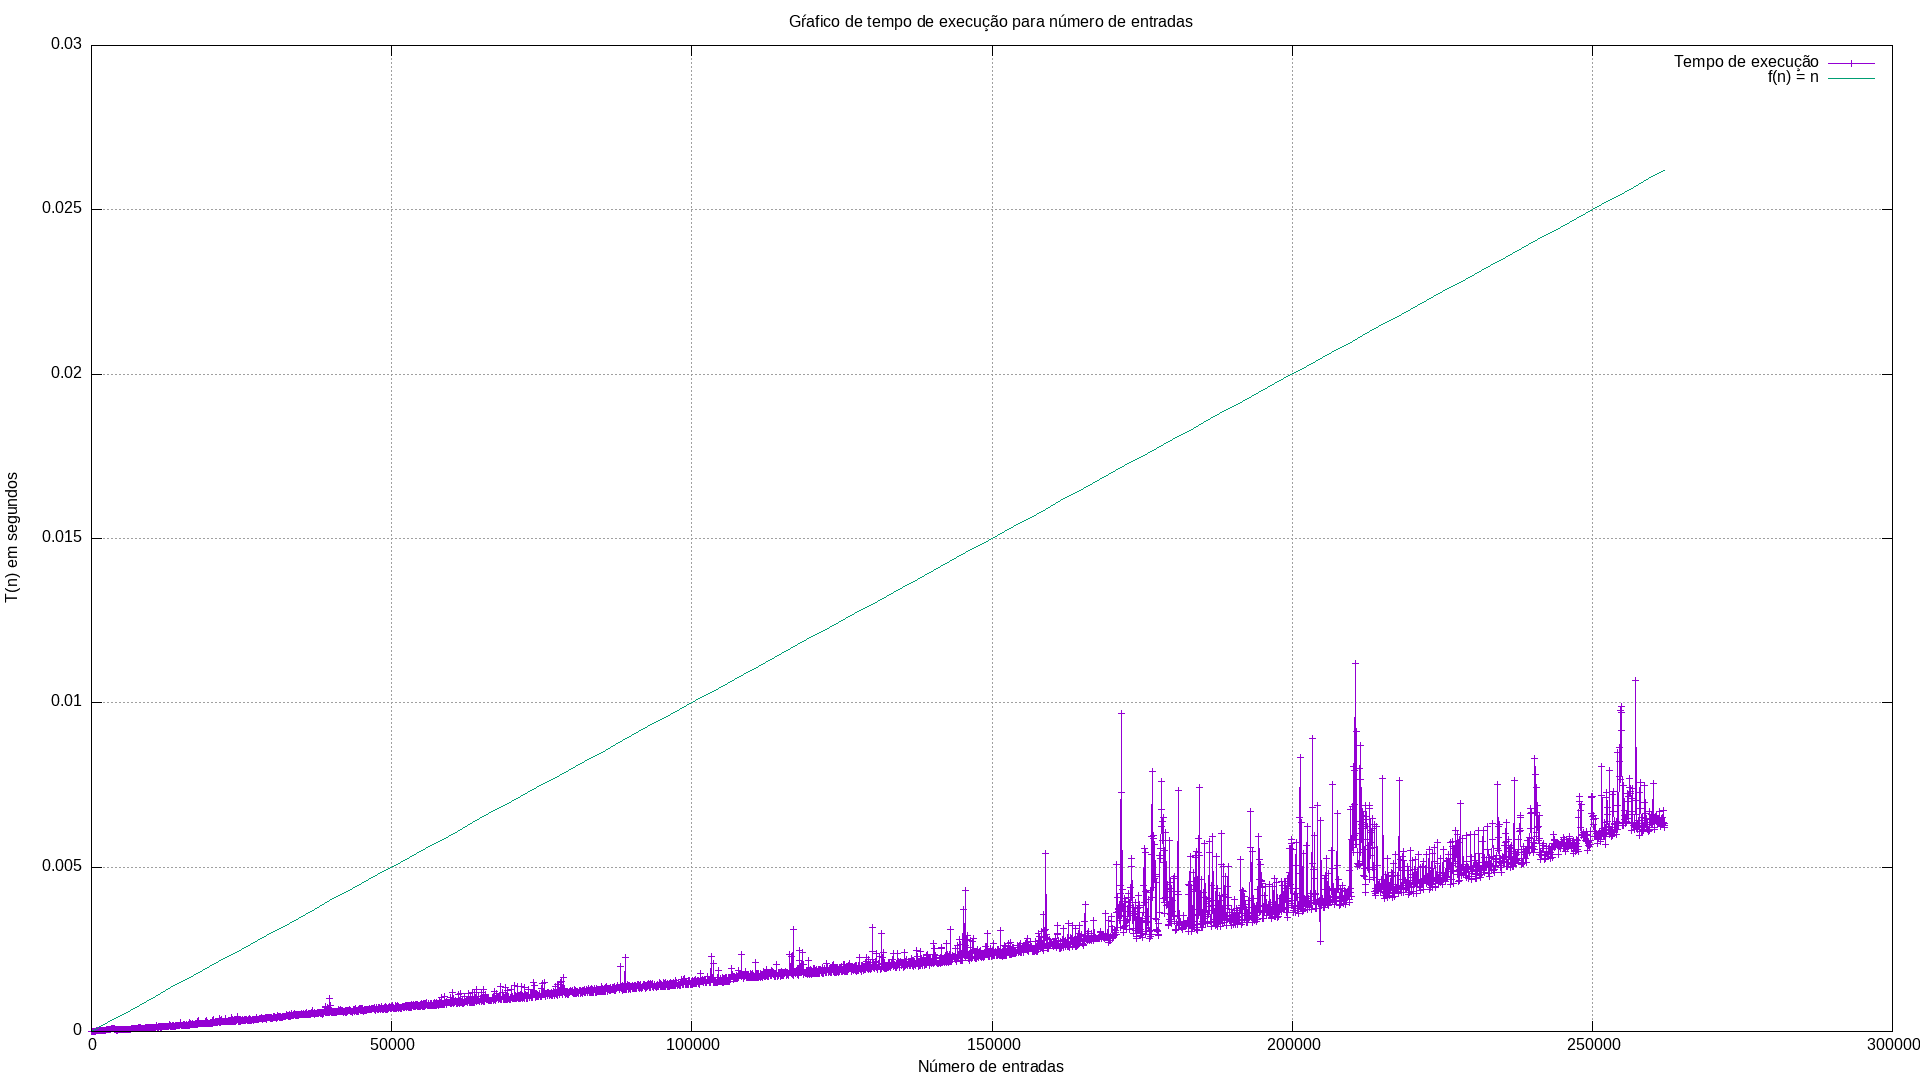
\includegraphics[width=\textwidth]{image/graphics/btree.png}
    \caption{Gráfico com tempo de execução do algoritmo de busca em árvore não-ordenada}
    \label{cap:3:graph:bTree}
\end{figure}

O gráfico obtido indica que:
